\section{The need for a new model}
\label{sec:literature_issues}

\subsection{Measuring MNCs' Activities}

For most of political science theory regarding FDI, the quantity of interest is the scale of MNCs' activities in a country, and not necessarily how much FDI crosses its border. Indeed, we theorize about how MNCs may reduce their activities for fear of expropriation, and how the host country's political factors can induce MNCs to invest more with a credible commitment not to expropriate. It is also the scale of MNCs' activities that determines how many jobs are created or how much of the domestic market is competed away, engendering labor's support and local business' lament.

However, to measure the scale of MNCs' activities, the vast majority of works uses how much FDI crosses the border, specifically FDI stock and flow \citep{Jensen2003, Ahlquist2006, Beazer2011, Graham2010}. As \citet{Kerner2014} points out, these measures, whose original purpose is to monitor balance of payments, are often misleading about MNCs' activities. FDI flow does not count locally raised capital and reinvested earnings since they do not cross any border. FDI stock calculated at market value fluctuates based on market price, unrelated to firms' behavior. FDI stock calculated at historical value, which records asset value at the time it was acquired, is more stable and appropriate to measure the scale of MNCs' activities. Unfortunately, due to onerous data requirements, most countries measures FDI stock by simply adding up FDI flow across years.

Given the interest of political science theory in MNCs' activities, \citet{Kerner2014} suggests less use of FDI stock and flow and more use of firm-level statistics. For example, consider the hypothesis that countries with more veto players have more stable policies and are thus more attractive to FDI \citep{Li2009a}. Instead of using FDI stock and flow into a country to measure its attractiveness, we can study whether more MNCs are located there.

While firm-level data has become more abundant in recent years,\footnote{Examples of firm-level data include the US Bureau of Economic Analysis (BEA)'s survey of all US firms abroad, Tokyo Keizai's Overseas Japanese companies database (\textit{Kaigai Sinshutsu Kigyou Souran}), World Bank's Enterprise Survey, and Orbis database of companies worldwide.} it is harder to analyze this type of data appropriately. Given the data structure of a set of firms interacting with a set of countries, one may consider a dyadic-based analysis, frequently used in the International Relations literature. In such analysis, the unit of observation is a firm-country dyad, and the model used is typically OLS regression. Each dyad is assumed to be independent of each other, and any bias caused by interdependency is fixed via post-estimation procedures, such as clustered standard errors \citep{Dorff2013}. 

Unfortunately, this dyadic approach is inappropriate to analyze MNCs' investment location. Once a firm chooses to invest in a country, it is by definition not investing in another. Therefore, the values of firm-country dyads deterministically constrained one another and cannot be modeled as independent draws from a common distribution.

The two sided matching model solves this problem by considering one firm-country match as the unit of observation. The intuition is that, if we observe that a firm is welcome to invest in countries $j_1, j_2, \dots, j_n$ but ends up investing in country $j^*$, it must mean country $j^*$ offers the highest utility to firms. Continuing the previous example, suppose that country $j^*$ has more veto players than average, we can infer that MNCs indeed prefer countries with more veto players.

\subsection{Estimating Countries' Demand for FDI}

Recognizing that our model of investment location has not taken into account countries' demand for FDI, \citet{Pinto2013} and \citet{Pandya2016} recently broke ground in this area. Similar to the rich IPE literature in trade and exchange rate, these studies argue that countries' demand for FDI varies according to FDI's distributive effect on their domestic constituencies \citep{Broz2001, Milner2005a}. In this theoretical framework, labor supports FDI because foreign firms bring capital that increases the demand for labor and raises productivity, both of which lead to higher wage. On the other hand, domestic firms oppose FDI because foreign firms compete for local labor, inputs, and markets. Both \citet{Pinto2013} and \citet{Pandya2016} formulate their theories as a variant of this labor-vs-business tension, which surfaces in the former work as left-vs-right governments, and in the latter as democratic-vs-authoritarian regimes.

While these pioneering works have enriched our understanding of the relationship between politics and FDI, their empirical approach does not satisfactorily measure countries' demand for FDI, leaving their theoretical arguments untested.

For example, consider \citet{Pinto2013}'s approach, which controls for economic and institutional factors that affect FDI flow into a country. The author then claims that the country's openness towards FDI is what's left in the residual.\footnote{Specifically, the estimation of FDI openness involves two steps. First, the author runs a gravity model explaining bilateral FDI flows, estimating the intercept as the host country-year fixed effect. Second, this fixed effect is then regressed on several economic and endowment factors of that country-year (i.e. GDP, GDP per capita, average school years, arable land). The residual in the second stage is considered the country's ``FDI openness'' in that year.} For this approach to be valid, every economic, institutional, and endowment factors that affect FDI flow have to be controlled for, leaving only the country's demand in the error term. This claim is much stronger than the regular assumption of exogenous and normally distributed error, which is valid as long as the omitted factors are uncorrelated with the independent variable of interest. Framed substantively, since the residual is likely to contain more than just the country's demand for FDI, if we observe an abnormally high level of FDI we do not know whether it is because the country welcomes FDI or because MNCs find something attractive in the country.\footnote{In addition, the data requirement of bilateral FDI flows, ideally disaggregated by sectors, is very demanding. Therefore, this approach is limited to OECD countries only \citep{Pinto2008}. During the period the authors study, 1980-2000, OECD countries accounted for 95\% of global FDI outflow and 90\% of inflow. However, since then the role of the developed world in global FDI has declined sharply, reduced to 60.8\% of outflow and 40.6\% of inflow in 2014 \citep{UNCTAD2015}.}

In contrast to \citet{Pinto2013}'s statistical approach, \citet{Pandya2014, Pandya2016} substantively measure countries' demand for FDI, using the annual US Investment Climate Reports to code how many industries in a certain country have foreign ownership restrictions or face investment screening. The advantages of this measurement is its ease of interpretation and its availability for many countries. However, two problems remain. First, adding up the raw count of restricted industries is not appropriate because industries are not all the same. For example, given the reach of the banking sector into all corners of the economy, a country's opening up its financial industry indicates much more FDI-friendliness than, say, allowing foreign furniture makers to set up shops. Since the theoretical argument is driven by FDI's distributive effect, it is suspect to ignore the varying impact of FDI across sectoral constituencies. 

Second, according to the coding rules, an industry is coded as free if there is no mention of restriction. If an industry receives little FDI, it may not be worth mentioning as being restrictive and yet still coded as open. Therefore, ``zero restriction'' in the dataset can either mean that a country is very closed or very open to FDI. This concern is not hypothetical. \Cref{fig:china_fdi_restriction} shows that, following the coding of the US Investment Climate Reports, China seemed 100\% open to FDI up until 1986 when it started imposing restrictions. The reality is opposite. Prior to 1986, 1only limited FDI is allowed as joint-venture in Special Economic Zones (SEZ). The year of 1986 was, in fact, the first time China allowed any wholly owned FDI outside of SEZs.

\begin{figure}[!ht]
\centering
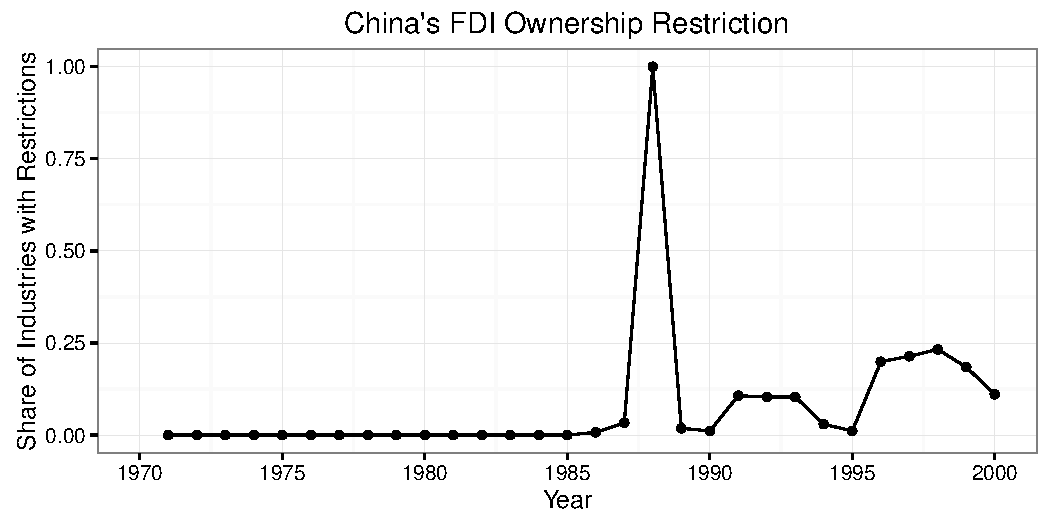
\includegraphics[width=0.75\textwidth,keepaspectratio]{../figure/china_fdi_restriction}
\caption{China's FDI Ownership Restriction, as coded in \citet{Pandya2010}. Prior to 1986, FDI in China was limited to few experimental Special Economic Zones, and thus not mentioned in US Investment Reports, designed for US firms. The sharp spike in 1988 also does not seem to correspond to any actual change in policy, and thus likely an artifact of reporting. See \citet{Zebregs2002} for a historical overview of China's FDI policy.}
\label{fig:china_fdi_restriction}
\end{figure}

The two-sided matching model circumvents these thorny measurement issues by incorporating countries' utility function directly into the model. The intuition is that, if we observe that country $j$ welcomes firms $i_1, i_2, \dots, i_n$ to invest but not others, we can compare the characteristics of firms $i_1, i_2, \dots i_n$ with the rest to infer country $j$'s preference.


\subsection{Estimating Countries' Preference for Specific FDI Characteristics}

While the political science literature has focused almost exclusively on the quantity of FDI, treating all FDI as one homogeneous flow of capital, policy makers seem to pay much more attention to distinguishing types of FDI. Commenting on the role of International Investment Agreements (IIAs), \citet{UNCTAD2015} says, ``Today, increasing the quantity of investment is not enough. What matters is its quality, i.e. the extent to which investment delivers concrete sustainable development benefits.'' Governments from Ireland, Ghana, to China all offer various forms of tax incentives and fee waivers to attract FDI that invests in a remote region, brings new technology, or focuses on exporting \citep{Ricupero2000}. Since 2006, China's official FDI policy has been ``quality over quantity,'' promoting FDI with intense R\&D in high-productivity sectors \citep{Guangzhou2011}.\footnote{All of these models also cannot investigate countries' preference for specific firms' characteristics. Pondya's look at cross industry, but because of data issue she can only do cross-sectional at the industry level instead of country-industry level. This level of aggregation is dubious: the same industry in one country is different from another country. For example, automobile value chain is vastly different across countries (example here). All of the industry estimates are based on US firms, which really cannot be realized to others. (It can for some basic industry characteristics / technology level, not for whether an industry is market oriented or not.)}

Disaggregating FDI has been a very difficult task. The few existing attempts can only use detailed data from one country or limit the sample to OECD countries \citep{Alfaro2003, Alfaro2007, Javorcik2004}. Using firm level data, this is not as challenging, but brings up the need for an appropriate model.

